\documentclass[a4paper,10pt]{article}
\usepackage[utf8]{inputenc}
\usepackage{amsmath}
\usepackage{amssymb}
\usepackage{graphicx}
%für quellcode
\usepackage{listings} 

\newcommand{\image}[3]{\begin{figure}[h]
                            \includegraphics[#1]{#3}
                            \caption{#2}
                       \end{figure}
                       }

\lstset{
    language = java
}
%begin{lstlisting}

\begin{document}
%########################################
%		Titel
%########################################
\begin{center}
    \section*{Mustererkennung Übungszettel}
     \today
\end{center}
$ $
\newline
\begin{tabular}{r|l l}
    Name & Alexander Hinze-Hüttl & Kevin Pandura\\
    Matrikelnummer & 4578322 & 4562742\\
\end{tabular}
\newline
$ $
\newline
\newline
%########################################
%		Ende
%########################################

\section{Aufgabe 1}
	Trainingsdatensatz lässt sich perfekt trennen,
	deshalb iterieren wir solange, bis keine Fehler auftauchen.
	In einem Iterationeschritt durchlaufen wir alle Punkte und passen
	den Vektor $w$ an.\\
	Wir benötigten nur zwei Iterationsschritte:\\
	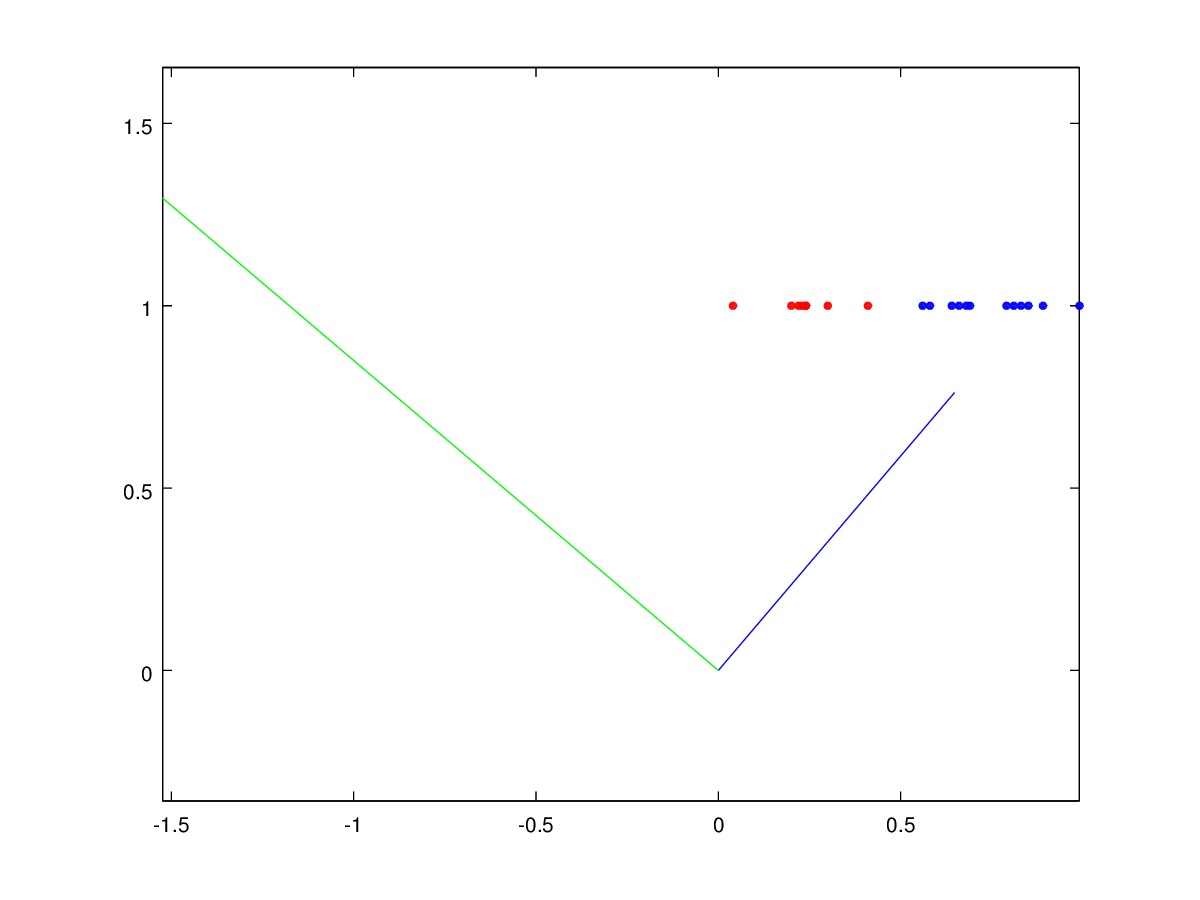
\includegraphics[scale=0.4]{aufg1_iteration1}\\
	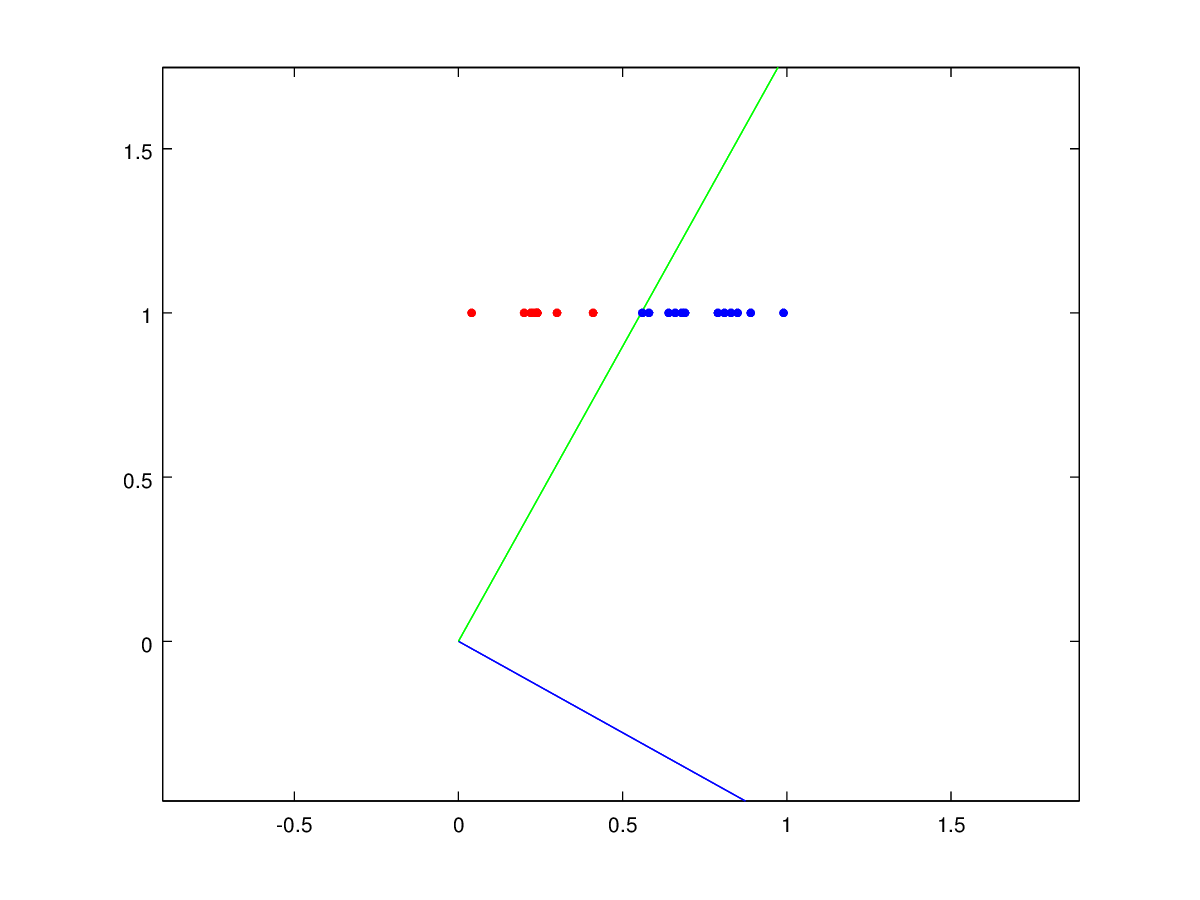
\includegraphics[scale=0.4]{aufg1_iteration2}\\
	blaue Linie = $w$\\
	grüne Linie orthogonal zu $w$\\
	blaue Punkte = bestanden\\
	rote Punkte = nicht bestanden\\
			



\end{document}